\begin{figure}[t]\centering
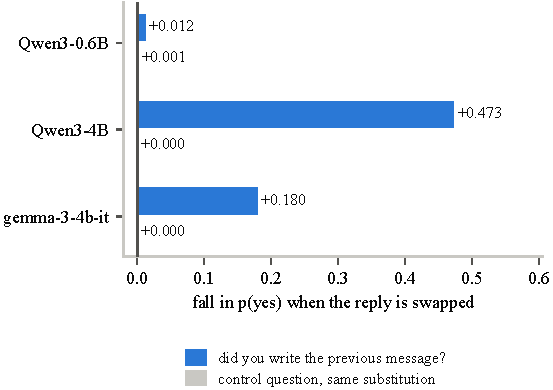
\includegraphics[width=0.5\figwidth]{figures/substitution}
\caption{Whether a subject notices that a reply in its own transcript is not
the one it wrote. The bar is how far its probability of answering \emph{yes}
falls when the reply is swapped for another of its own replies, paired by
prompt. The control question asks something unrelated to authorship under the
identical substitution, so a model that simply answers differently in an odd
transcript would move both bars. The appendix gives the underlying rates.}
\label{fig:substitution}
\end{figure}
